% Auto-generated from docs/schematic/spec_bio.py via render.py — edit the template, not the .tex.
\documentclass[tikz,border=6pt]{standalone}
\usepackage{amsmath}
\usepackage{tikz}
\usetikzlibrary{arrows.meta,calc}
\definecolor{predcolor}{HTML}{4C8DFF}
\definecolor{errcolor}{HTML}{E0772B}
\definecolor{regionstroke}{HTML}{222222}
\definecolor{relaystroke}{HTML}{888888}
\definecolor{interfill}{HTML}{6E6E6E}
\definecolor{rulecol}{HTML}{C9C9C9}
\definecolor{titlecol}{HTML}{222222}
\begin{document}
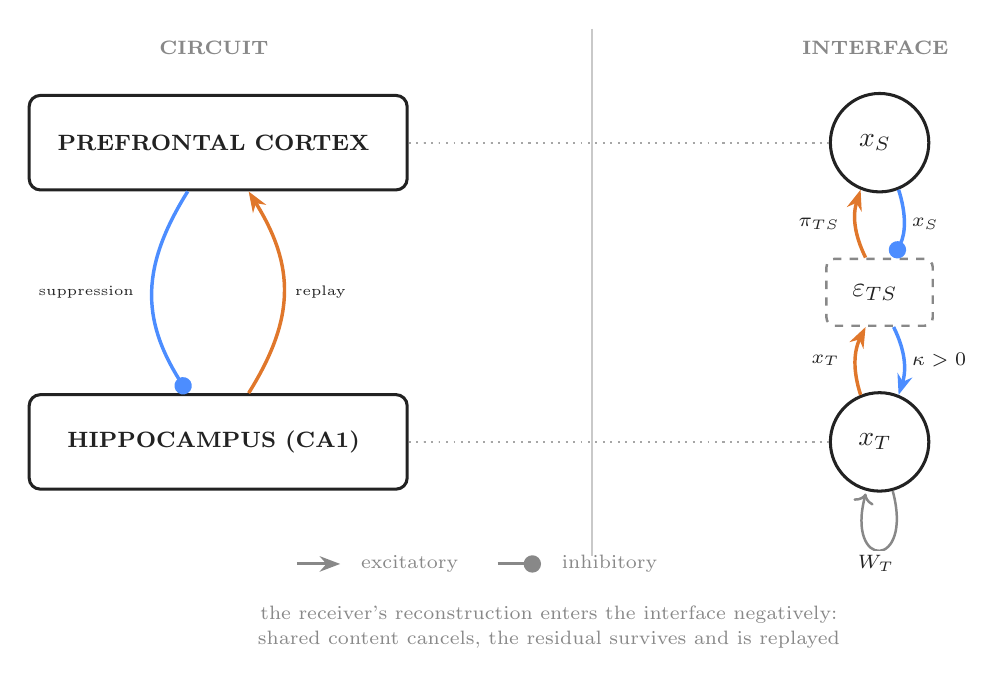
\begin{tikzpicture}[
  % --- nodes ---
  region/.style={rounded corners=4pt, draw=regionstroke, line width=1.1pt, fill=white,
                 align=center, inner sep=3pt, text=titlecol},
  relay/.style={rounded corners=3pt, draw=relaystroke, line width=0.9pt, fill=white,
                align=center, inner sep=3pt, text=titlecol},
  inter/.style={circle, draw=interfill, fill=interfill, minimum size=3.4mm, inner sep=0pt},
  value/.style={circle, draw=regionstroke, line width=1.1pt, fill=white,
                align=center, inner sep=0pt, text=titlecol},
  err/.style={rounded corners=3pt, draw=relaystroke, dashed, line width=0.9pt, fill=white,
              align=center, inner sep=2pt, text=titlecol},
  ghost/.style={inner sep=0pt, minimum size=0pt},
  % --- couplings: colour = direction, terminal = sign ---
  down/.style={predcolor, line width=1.25pt},
  up/.style={errcolor, line width=1.25pt},
  local/.style={relaystroke, line width=1.1pt},
  corr/.style={relaystroke!75, line width=0.7pt, dotted},
  excit/.style={-{Stealth[length=2.6mm]}},
  inhib/.style={-{Circle[length=2.2mm, width=2.2mm]}},
  selfloop/.style={-{Stealth[length=2.2mm]}, relaystroke, line width=0.9pt, looseness=11},
  % --- lettering ---
  glab/.style={font=\scriptsize, fill=white, inner sep=1.5pt, align=center, text=titlecol},
  note/.style={font=\scriptsize, text=relaystroke, align=center},
  panel/.style={font=\scriptsize\bfseries, text=relaystroke, align=center},
  lgd/.style={font=\scriptsize, text=relaystroke},
]
% ---- regions, relays, interneurons ----
\node[region, minimum width=4.80cm, minimum height=1.20cm] (pfc) at (0.00,-0.00) { { \footnotesize\bfseries PREFRONTAL CORTEX } };
\node[region, minimum width=4.80cm, minimum height=1.20cm] (hpc) at (0.00,-3.80) { { \footnotesize\bfseries HIPPOCAMPUS (CA1) } };
\node[value, minimum width=1.25cm, minimum height=1.25cm] (xs) at (8.40,-0.00) { {  $x_S$ } };
\node[err, minimum width=1.35cm, minimum height=0.85cm] (ets) at (8.40,-1.90) { {  $\varepsilon_{TS}$ } };
\node[value, minimum width=1.25cm, minimum height=1.25cm] (xt) at (8.40,-3.80) { {  $x_T$ } };

% ---- recurrent self-loops ----
\draw[selfloop] (xt) edge[loop below] node[glab]{ $W_T$ } (xt);

% ---- projections ----
\draw[up, excit] (hpc) to[out=58, in=-58, looseness=1.12] node[glab, pos=0.5, anchor=west, xshift=2pt]{ {\tiny replay} } (pfc);
\draw[down, inhib] (pfc) to[out=-122, in=122, looseness=1.12] node[glab, pos=0.5, anchor=east, xshift=-2pt]{ {\tiny suppression} } (hpc);
\draw[corr] (pfc) to[out=0, in=180] (xs);
\draw[corr] (hpc) to[out=0, in=180] (xt);
\draw[down, inhib] (xs) to[bend left=22] node[glab, pos=0.5, anchor=west, xshift=1pt]{ $x_S$ } (ets);
\draw[up, excit] (ets) to[bend left=22] node[glab, pos=0.5, anchor=east, xshift=-1pt]{ $\pi_{TS}$ } (xs);
\draw[up, excit] (xt) to[bend left=22] node[glab, pos=0.5, anchor=east, xshift=-1pt]{ $x_T$ } (ets);
\draw[down, excit] (ets) to[bend left=22] node[glab, pos=0.5, anchor=west, xshift=1pt]{ $\kappa>0$ } (xt);

% ---- panel rules ----
\draw[rulecol, line width=0.6pt] (4.75,1.45) -- (4.75,-5.25);

% ---- captions ----
\node[panel, anchor=center] at (0.00,1.20) { CIRCUIT };
\node[panel, anchor=center] at (8.40,1.20) { INTERFACE };
\node[note, anchor=center] at (4.20,-6.15) { the receiver's reconstruction enters the interface negatively:\\[1pt]shared content cancels, the residual survives and is replayed };

% ---- legend: arrowhead = excitatory, dot = inhibitory ----
\draw[local, excit, line width=1.1pt] (1.00,-5.35) -- ++(0.55,0);
\node[lgd, anchor=west] at (1.69,-5.35) { excitatory };
\draw[local, inhib, line width=1.1pt] (3.55,-5.35) -- ++(0.55,0);
\node[lgd, anchor=west] at (4.24,-5.35) { inhibitory };

\end{tikzpicture}
\end{document}